\section{Images} 

  A pixel can be really represented by a number. More specifically, a grayscale pixel is a number between $0$ (black) and $255$ (white), and a color pixel is in the RGB format, represented by a $3$-tuple. Therefore, a grayscale image is really represented by a $H \times W$ matrix, and a RBG image by a $3 \times H \times W$ tensor. We can see this when opening up an image in OpenCV with the following code: 
  \begin{lstlisting}
    import cv2 

    PATH = "park.jpg"

    img = cv2.imread(PATH)
    gray = cv2.cvtColor(img, cv2.COLOR\_BGR2GRAY) 

    cv2.imshow("Park", img)     # Show RGB image
    cv2.imshow('Gray', gray)    # Show gray image
    cv2.waitKey(0)              # Wait time until image closes
  \end{lstlisting}

  The results are shown in the figure below.

  \begin{figure}[H]
    \centering
    \begin{subfigure}[b]{0.45\textwidth}
    \centering
        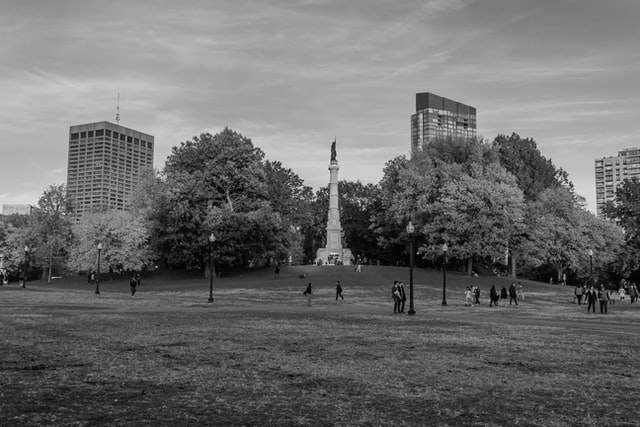
\includegraphics[width=\textwidth]{img/Gray_Full.png}
        \caption{Gray picture of park}
        \label{fig:1d}
    \end{subfigure}
    \begin{subfigure}[b]{0.45\textwidth}
    \centering
        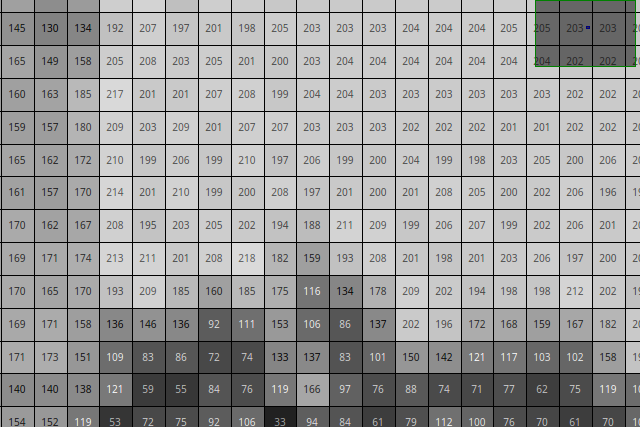
\includegraphics[width=\textwidth]{img/Gray_Cropped.png}
        \caption{Gray channel}
        \label{fig:2d}
    \end{subfigure}

    \centering
    \begin{subfigure}[b]{0.45\textwidth}
    \centering
        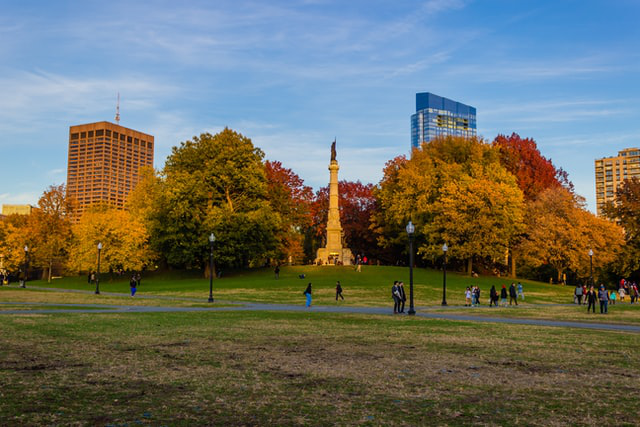
\includegraphics[width=\textwidth]{img/Park_Full.png}
        \caption{Colored picture of park}
        \label{fig:3d}
    \end{subfigure}
    \begin{subfigure}[b]{0.45\textwidth}
    \centering
        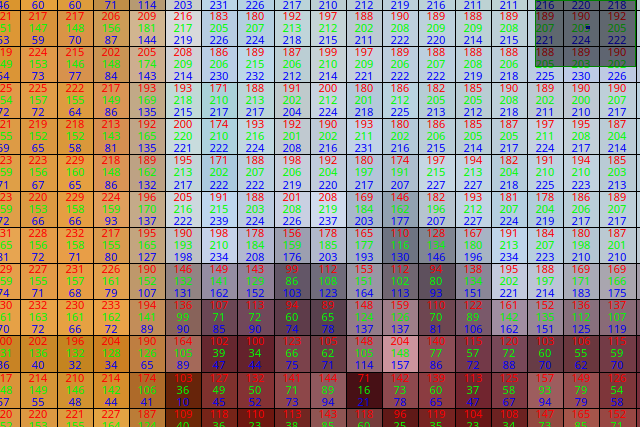
\includegraphics[width=\textwidth]{img/Park_Cropped.png}
        \caption{RGB channels}
        \label{fig:4d}
    \end{subfigure}
    \label{fig:Park_Images}
    \caption{Different color channel representations of an image. }
  \end{figure}

  The $\texttt{img}$ object called by $\texttt{cv2.imread()}$ actually outputs a numpy array directly. This makes it easy for us to access the resolution of the image and to crop it by slicing across the dimensions. We can also rescale it accordingly using $\texttt{cv.resize()}$. 
  \begin{lstlisting}
    print(img.shape)        <class 'numpy.ndarray'> (427, 640, 3)
    print(gray.shape)       <class 'numpy.ndarray'> (427, 640)

    # Crop it 
    img\_cropped = img[100:200, 100:200, :]

    # Resize the image 
    width, height = int(frame.shape[1] * 0.6), int(frame.shape[0] * 0.6) 
    dimensions = (width, height) 
    img\_resized = cv2.resize(img, dimensions, interpolation=cv2.INTER\_AREA) 
  \end{lstlisting}

\subsection{Color Histograms}

  You can also find the distribution of the color channels in an image with a histogram. A code snippet is shown below, along with the corresponding generated plots in the figure below. 

  \begin{figure}[H]
    \centering
    \begin{subfigure}[b]{0.45\textwidth}
    \centering
        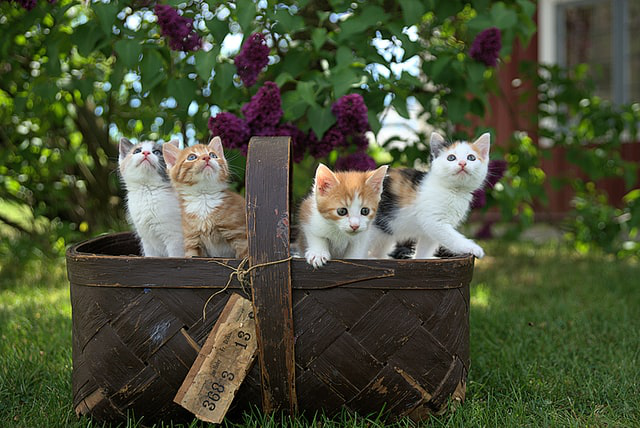
\includegraphics[width=\textwidth]{img/Cats.png}
        \caption{Gray picture of park}
        \label{fig:5d}
    \end{subfigure}
    \begin{subfigure}[b]{0.45\textwidth}
    \centering
        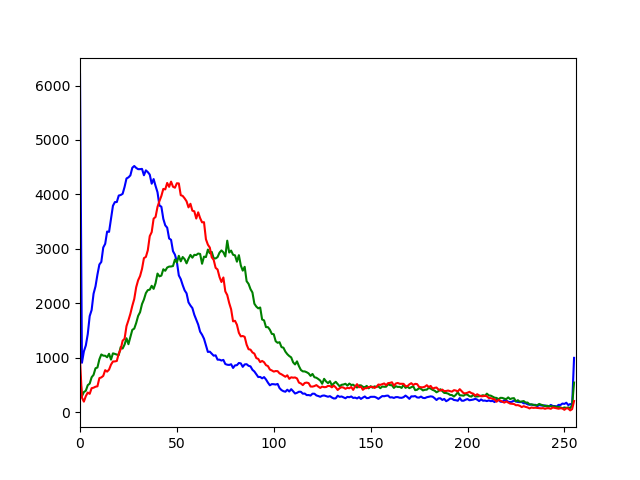
\includegraphics[width=\textwidth]{img/Cats_color_hist.png}
        \caption{Gray channel}
        \label{fig:6d}
    \end{subfigure}
    \label{fig:cats_histogram}
    \caption{RBG Channel Histograms for Cats.png image. }
  \end{figure}

  \begin{lstlisting}
    img = cv2.imread("Cats.jpg")
    cv2.imshow("Cats", img) 

    # Color histogram 
    colors = ('b', 'g', 'r') 
    for i, col in enumerate(colors): 
        hist = cv2.calcHist([img], [i], None, [256], [0, 256]) 
        plt.plot(hist, color=col) 
        plt.xlim([0, 256]) 
        
    plt.show() 
    cv2.waitKey(0) 
  \end{lstlisting}

\subsection{Camera Parameterization} 

